% !TEX root = ../thesis.tex
%
\chapter{Evaluation}
\label{sec:evaluation}

\section{Runtime Benchmarks}
\label{sec:evaluation:runtime_benchmarks}

Over the course of this thesis two different approaches to handling the progress of streams in the runtime were explored, which were briefly mentioned in Chapter~\ref{sec:definitions:run}: progress timestamps and progress events.
Progress timestamps were used first, which worked, but lead to big overhead when a great number of computations had to happen, since the whole stream had to be send to all children of the node that performed the computation.
Therefore later the runtime was refactored to use progress events, so that only events had to be sent between nodes.
The following benchmarks will show the performance characteristics of both approaches under different circumstances.

\subsection{Number of Processors}

Since one of the main motivations to choose erlang and BEAM as the plattform for the runtime was its support for parallel execution on many processor cores, in this section the performance characteristic in regard to available cores is explored.
To do so a simple \gls{tessla} specification is given, that includes as many nodes as the maximal number of processors available.
Such a spec for eigth processors is given in Listing~\ref{listing:runtime_parallel_spec_8}.

\begin{figure}
  \lstinputlisting[caption=\gls{tessla} specification with eight nodes on the critical path,label=listing:runtime_parallel_spec_8]{content/code/parallel_8.spec}
\end{figure}

The specification is evaluated over appropriate traces with a specified amount of processor cores available.
The needed time of the evaluation engine from its start until it emits the conclusion, that the stream \(\mathit{done}\) is \(\mathit{true}\), is measured for different amounts of processors.
All benchmarks were performed with upto 16 cores and 50GB of RAM.

One thing that showed during benchmarking was, that the older implementation approach used big amounts of RAM and the usage growed exponential with the amount of used cores.
For example with two used cores the runtime would use around 2GB RAM, with 4 Cores already over 8GB.
This can be explained easily: since in the old implementation all data has to be sent between all cores while in the new implementation only generated events have to be sent around.
The excessive usage of RAM even lead to timeout under some circumstances and crashes the whole runtime.
The amount of data send between processes can even lead to negative performance impacts when more cores are added.

This behaviour was one of the main reasons to switch to a new approach.
To test if reduced RAM usage would lead to better performance and eliminate crashes, the old architecture was changed in a small way: Each stream was limited to only hold the last 20 events, all older events were thrown away.
Since the specification used for benchmarking only works on the most recent event of each stream, this would not alter the conclusion of the engine.
For example a specification computing the average of the last 21 events wouldn't work with this adaption.

While the RAM usage of the adapted runtime is not shown, the performance impact is obvious.
Thus the new architecture was implemented.

TODO: describe how V2 scales with core number.

Figure~\ref{fig:chap_eval:runtime_parallel} shows the performance characteristics of both implementations and the adapted implementation in regard to used processor cores.

\subsection{Number of Events}
TODO: also show memory consumption!
\subsection{Number of Nodes}

\section{Practical Examples}
\label{sec:evaluation:runtime_examples}

Additionally to the theoretic benchmarks it was also important to evaluate the runtime against some more practical examples.
Therefore some traces from real world examples were collected, either with the instrumentation pass or by adjusting existing logs to fit the needs of \gls{tessla}.
The programs or traces were then modified to deliberately include errors to test if appropriate \gls{tessla} specifications will find them when evaluated in the runtime.

\subsection{Ringbuffer Examples}

The main source for tests is a ringbuffer, implemented in C, which was then modified by the instrumentation to generate traces.
The code of the ringbuffer can be found in Chapter~\ref{sec:appendix:ringbuffer}.



\section{Instrumentation Benchmarks}
\label{sec:evaluation:instrumentation_benchmarks}

After the evaluation of the runtime itself it remains to evaluate the C instrumentation program.
Note that the instrumentation is mostly a proof of concept and its main purpose for now was to generate test data for the runtime.
But it seems feasible that it can be optimized and extended to become a general purpose trace collection tool, therefore some benchmarks were performed.

For reliable trace collection of software the performance impact of the instrumentation is important.
To measure this a trivial C programm was benchmarked with and without instrumentation.
The program increments each integer from 0 to 100000000 by one and, if the incremented number is divisible by a given parameter \(c\), adds it to an intermediate result.
Note that the programm  can and will perform some integer overflows.
The code is shown in Listing~\ref{listing:instrument_benchmark_code}.

\begin{figure}
\lstinputlisting[language=c, label=listing:instrument_benchmark_code, caption=Example C program for benchmark purposes]{content/code/instrument_benchmark.c}
\end{figure}

The code is then instrumented to log each call of the \lstinline{add} method.
For each benchmark the compiled program was run 50 times.
All benchmarks were performed on an Intel Core i5 with two cores and 8GB of Ram.
The complete dataset can be found in Chapter~\ref{sec:appendix:instrumentation_benchmark_data}.

\subsection{Performance Comparison with non Instrumented Code and Compiler Optimizations}
\label{sec:evaluation:instrumentation_benchmark:instr_vs_non_inst}

One interesting metric is, how an instrumented program performs in contrast to the same program without the added instrumentation.
For this the parameter \(c\) is set to 100, so that around 1\% of all function calls are instrumented.

One thing that can be recognized is that the impact of instrumentation is not predictable when using compiler optimizations.
Aggressive compiler optimizations can remove function calls or inline values if it doesn't change the programs behaviour.
When instrumentation calls are added no such optimization can happen, since else behaviour of the program would be altered, namely the logging would be removed when the function calls are removed.

Therefore we compare the instrumented and non-instrumented code for all optimization levels.
The comparison can be seen in Figure~\ref{fig:chap_eval:instrument_benchmark_results}.

\begin{figure}
  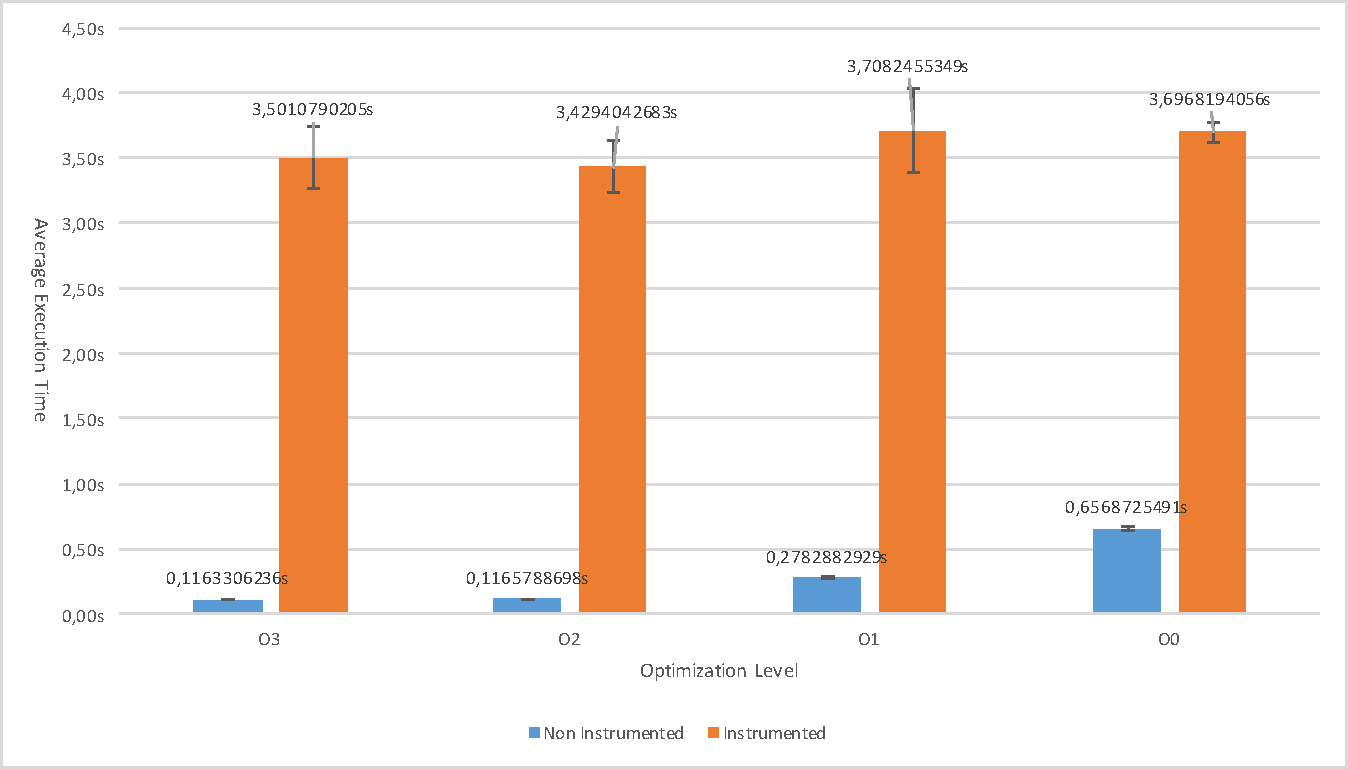
\includegraphics[angle=90,origin=c,width=\textwidth]{gfx/instrumentation_benchmark}
  \caption{Performance of an example C program with and without instrumentation}
\label{fig:chap_eval:instrument_benchmark_results}
\end{figure}

The choice to instrument around 1\% of function was arbitrarily, after some experimentation showed that higher amount lead to huge performance impacts as shown in Chapter~\ref{sec:evaluation:instrumentation_benchmark:instr_amount}.
Intuitively it sound reasonable that in a real life example only a small subset of function calls are interesting for trace generation, since \gls{tessla} specifications should be used to monitor critical parts of a system.

\subsection{Performance Impact in Regard to Instrumentation Percentage}
\label{sec:evaluation:instrumentation_benchmark:instr_amount}

To further investigate the impact of instrumentation we will look at the performance impact in regard to the percentage of function calls that are instrumented.
Therefore the variable \(c\) of the program is changed, which leads to different amount of calls to the instrumented function.
For all values the program was compiled with the maximal optimization setting.
In Figure~\ref{fig:chap_eval:instrument_benchmark_amount_results} the results of changing the parameter can be seen.

\begin{figure}
  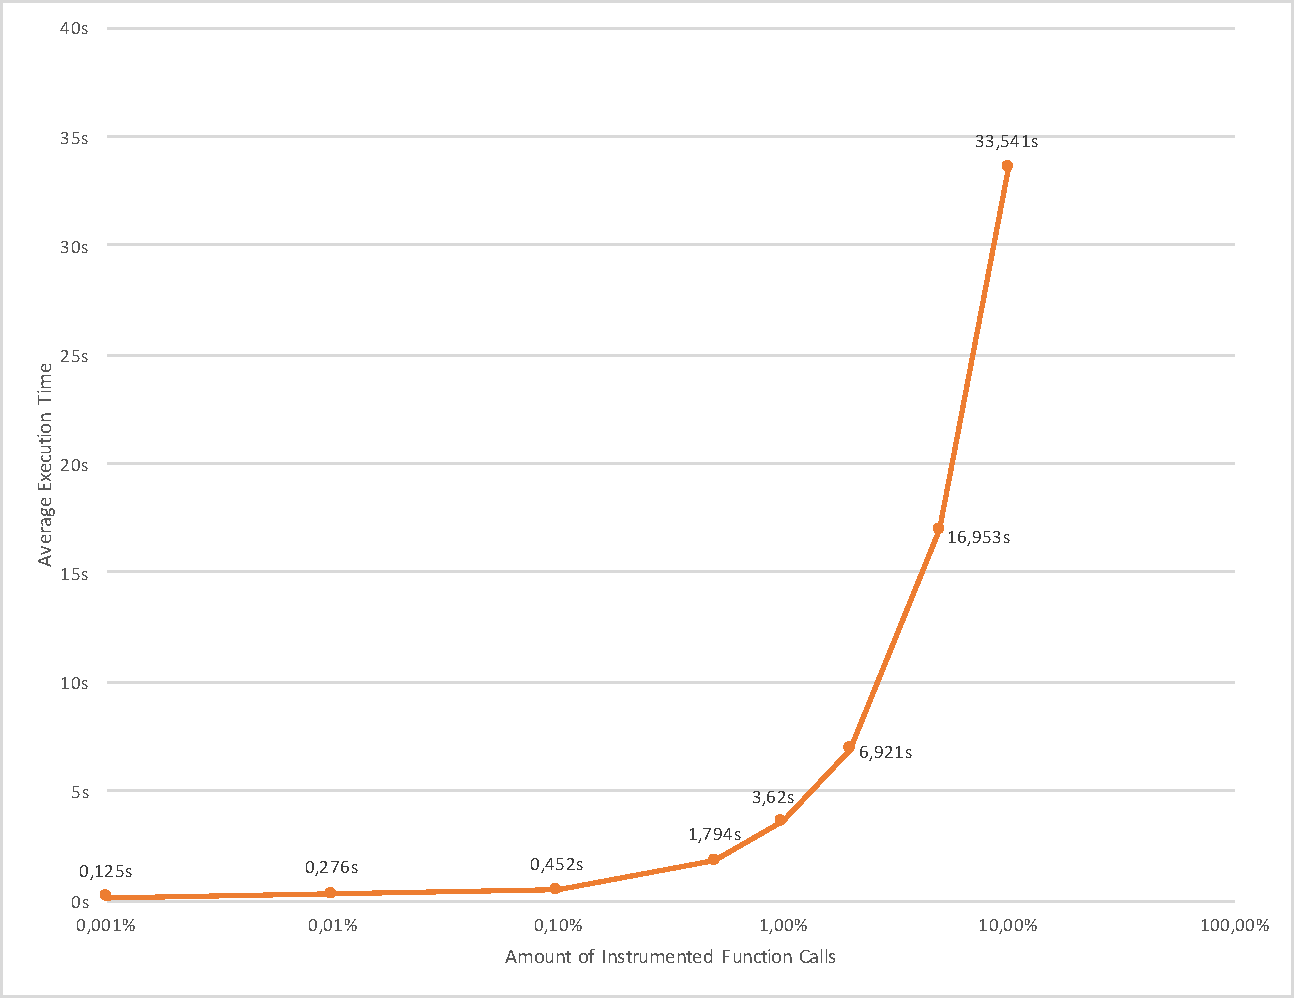
\includegraphics[width=\textwidth]{gfx/instrumentation_amount_benchmark.pdf}
  \caption{Execution time of a program with different amount of calls to an instrumented function}
\label{fig:chap_eval:instrument_benchmark_amount_results}
\end{figure}

Note that the x-axis is logarithmic.
As expected the performance impact scales directly with the amount of calls to the instrumented function.
At some point no more speed up will happen, since no calls to the instrumented functions will be made.

\subsection{Conclusion for the Instrumentation}

It can be seen, that the instrumentation adds a lot of overhead, especially when compiler optimizations are turned on and the amount of instrumented function calls are big.
While the overhead is big, it is stable (see the standard deviation in Chapter~\ref{sec:evaluation:instrumentation_benchmark:instr_vs_non_inst}).
This leads to the following conclusions: The generated traces should be mostly used for analysing test settings, where compiler optimizations are turned off.
When used for timing specifications, the instrumented code can be benchmarked against a non instrumented version of it and the results can be used to transform the actual timing requirements to ones for the instrumented code.
This will at least give an approximation of actual results.
ALso it is recommended to write small and specific \gls{tessla} specifications, so that the instrumentations only have to be applied to a small amount of functions.
Obviously it is strongly discouraged to use the instrumented code in any production setting.

